\chapter{Analytics in use}~\label{chapter-analytics-in-use}

This chapter presents the research findings based on two of the six perspectives: \uuse and \iuse, \emph{i.e.} how app developers currently use mobile analytics and ways the use could be improved. Figure \ref{fig:dev-practices-with-mobile-analytics} provides the visual context of the development practices and artefacts~\footnote{This figure will be revised pre-submission and keyed into the contents of this chapter. Versions of this figure may feature throughout the thesis with the pertinent elements highlighted and less relevant elements diminished or hidden from view.}.

\begin{figure}
    \centering
    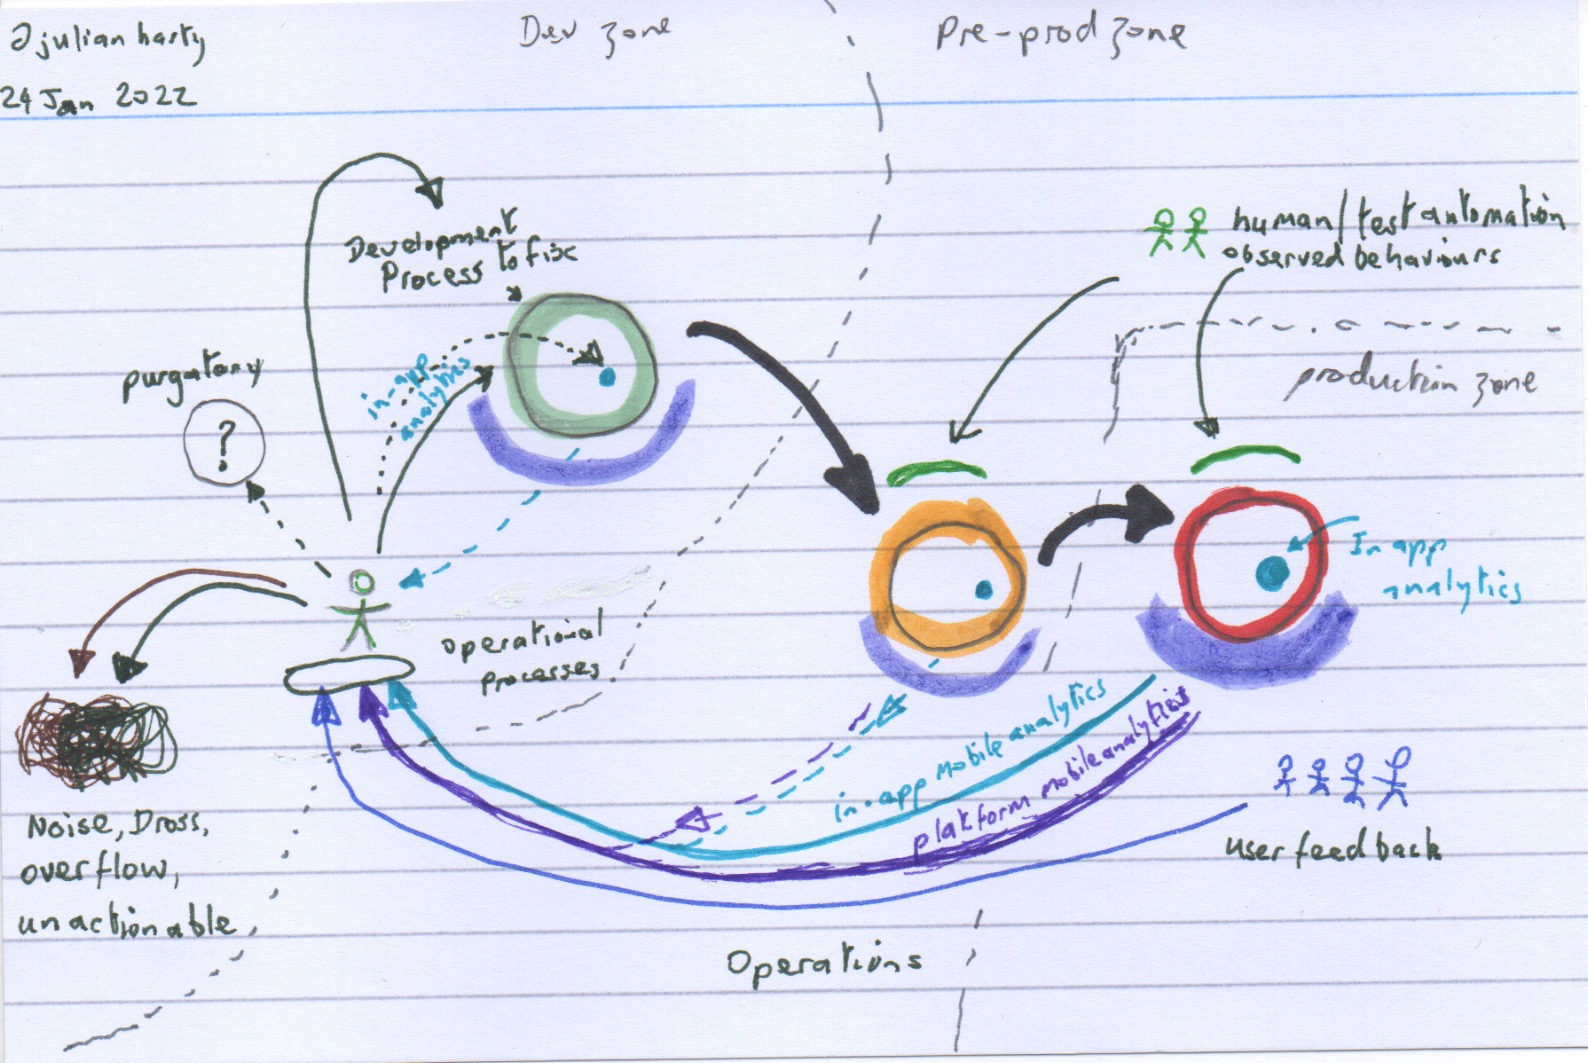
\includegraphics[width=12cm]{images/rough-sketches/dev-practices-with-mobile-analytics-24-jan-2022.jpeg}
    \caption{Dev Practices with Mobile Analytics}
    \label{fig:dev-practices-with-mobile-analytics}
\end{figure}

\julian{TODO introduce the rest of this chapter. Here's my current running order: \href{aiu-motivating-factors-section}{Motivation}, \href{aiu-choosing-mobile-analytics-section}{selection}, \href{aiu-application-of-mobile-analytics-section}{application}, 
\href{aiu-bug-reproduction}{bug reproduction}, 
\href{aiu-triage-section}{triage}, 
blockers,  
\href{aiu-snafu-and-real-world-conditions-section}{SNAFU and real-world conditions}, }

\section{Motivating factors}~\label{aiu-motivating-factors-section}
What motivates the development teams to pay attention and address failures reported by mobile analytics? The motivation may be viewed as a bi-directional continuum: at one end there is the wish to avoid and restrict failures that affect end users of the apps, at the other end there are desires to improve apps, engineering practices, including improving the use of mobile analytics. Fixing failures may be more tactical, while desiring improvements may be more strategic and involve a longer-term perspective.

In terms of the app-centric case studies only one of the interview-based studies - \href{glossary-gtaf}{GTAF} - explicitly explained they had periods of fixing high crash rates. Several of their Android apps had experienced high crash rates which had adversely affected the user experience. The project team have learned the importance of paying attention to crashes being reported by mobile analytics tools. They also realised the importance of addressing high crash rates. Accordingly, the development team used outputs from mobile analytics to identify the most frequent crashes they wanted to fix. In contrast, the majority of the rest of the interview-based studies were predominantly working to maintain good quality, to varying degrees based on their active and ongoing use of mobile analytics. The one odd-ball project was LocalHalo where the CTO appeared to only use mobile analytics infrequently despite having actively integrated several in-app analytics tools into their app and server codebases.

All of the action research-based app centric case studies were prompted by excessively high crash rates \emph{i.e.} they acknowledged they wanted/needed help both to tame the high crash rates and to improve the rates further on an ongoing basis.

For Kiwix, there was a pernicious, insidious increase in the crash rates for several of the most popular Android apps. The project leads particularly wanted to reduce the crash rates for the worst offenders in terms of the apps. Similarly the crash rate for Pocket Code far exceeded the bad behavior threshold, of 1.09\%, and despite the various recommended software development practices the project team had not been able to tame the excessive crash rate.

For the commercial app, it had a user-base of millions however bouts of issues in several releases of the Android app meant the app had significantly exceeded the bad behavior threshold, of 1.09\%, Google applies to all Android apps in the Google Play Store. They needed to solve the tactical issues in parallel with improving the engineering practices to reduce the likelihood of similar bouts and to encourage ongoing and long-lasting improvements to the quality of their app and the service. 

The commercial app-centric case studies all incorporated general purpose usage analytics into their apps in addition to error reporting, Firebase Analytics was the most popular choice, which is congruent with Firebase Analytics being the dominant market leader~\citep{appbrain_firebase}. LocalHalo chose Sentry, in part as it integrated well with React-Native, the cross-platform development framework they used for their mobile app.

The use of additional general purpose analytics is not confined to the commercial apps, Greentech apps team demonstrated how they had actively used mobile analytics to reduce the crash rate of their key apps and announced their intention to increase their use of mobile analytics in order to improve the user experience of their apps~\citep{gtafblog2021_gtaf_accomplishment_2020}. 


\section{Choosing Mobile Analytics}~\label{aiu-choosing-mobile-analytics-section}

\julian{TODO expand on selection and choosing}
The choice of which mobile analytics tools to use is in some ways a recursive characteristic. Firstly, there is the choice of whether to include any analytics within the app at all - the Kiwix project team chose not to in order to maximise the protection of end users' privacy and minimise the potential for repressive authorities finding and then abusing usage-related data to penalise end users of Wikipedia and similar material. The rest of the app-centric case studies included at least one in-app mobile analytics SDK in their app.

Some of the projects, including LocalHalo, Greentech apps, and the Commercial project, choose to incorporate several mobile analytics SDKs in their apps. Their reasons differed, for example LocalHalo used Mixpanel for business analytics and Sentry for technology-related analytics including crash reporting. Greentech apps appears to let each app developer decide on which mobile analytics service to incorporate. The corporate projects reasons were multi-factoral and outside the scope of the research.

Choices of SDK may change over time: for example the Catrobat project chose to remove in-app analytics from their flagship Pocket Code app as the replacement for the Fabric Crashlytics SDK also collected and combined PII data with the crash reporting. Like the Kiwix project team they wanted to err on protecting the privacy of their users (which includes many school-age children) and reduce their contributions to the already vast digital footprint owned by global tech superpowers.

Secondly, there is the choice of which source to use for which purposes. For instance both Android Vitals and the many crash reporting SDKs report on app crashes. All the projects who used in-app mobile analytics for crash reporting preferred to use that service to monitor the crashes in their app, even if some crashes aren't reported in that tool, for example those that occur as the app is starting up. Of the development teams who used in-app crash reporting Moonpig were unusual as they \textit{also} actively and frequently used Android Vitals to monitor crashes and other failures.

Thirdly, there are choices to be made in terms of what to record and when to do so in terms of in-app mobile analytics. Various in-app mobile analytics SDKs provide facilities for error reporting in addition to crash reporting. Broadly errors in this context are connected to caught and handled Java exceptions~\footnote{For avoidance of doubt this includes Kotlin and other JVM languages, errors reported in frameworks such as React Native, and caught signals in C++ code.}. Some SDKs include API calls to provide trails of `breadcrumbs' that lead up to an error or a crash~\footnote{For instance, see \url{https://www.bugsnag.com/blog/android-breadcrumbs-support}.}. None of the app-centric case studies mentioned actively using these breadcrumbs, however the reports Sentry generated for the LocalHalo app indicate the Sentry SDK generated automatic breadcrumbs~\footnote{\url{https://docs.sentry.io/platforms/react-native/enriching-events/breadcrumbs/}} and these helped identify the server was no longer functioning correctly in late 2021. 

%%%% Sources include: 
%%%%%%% https://www.bugsnag.com/blog/error-handling-on-android-part-7 
%%%%%%% https://github.com/backtrace-labs/backtrace-android
%%%%%%% https://backtrace.io/
%%%%%%% https://saucelabs.com/platform/error-reporting (which also mentions triage)
%%%%%%% For breadcrumbs several are listed in https://www.google.com/search?q=breadcrumb+crash+reporting+android 

Caught exceptions, signals, etc. are not the only form of error that might be of interest to developers. Projects including Smartnavi and Moonpig used general purpose mobile analytics for reporting additional errors, for instance that affected the user experience. Similarly the general purpose mobile analytics and the crash reporting SDKs both collect contextual and runtime information and developers sometimes use this information. Some additional joint research studied 107 actively maintained opensource Android apps hosted on GitHub, a topic we cover next.

\subsection{Developer-controlled characteristics}
\julian{TODO expand on the following:}
TODO discuss the initial config, and `getting started', then the optional additional use of the mobile analytics SDK's APIs. Provide examples from the log analysis research where 50 of 107 projects only used the minimal default initialisation rather than calling the rest of the Firebase Analytics API. 

TODO Mention the Pocket Code experience when migrating from Fabric to Firebase and the additional, unexpected analytics that appeared. Forward reference to the discussion on intrusiveness. 


\section{Application of mobile analytics}~\label{aiu-application-of-mobile-analytics-section}

\julian{Include horses-for-courses,...} 
As mentioned previously, several projects including LocalHalo chose to use a particular mobile analytics service for   business analytics. Pricing may also be a factor in the choice of SDK and service, however this topic was not actively discussed as part of the case studies.

\section{Bug reproduction}~\label{aiu-bug-reproduction}
Being able to reproduce bugs, ideally at-will, enables developers to work more effectively at addressing the bug and having confidence that their intended fixes actually do fix the bug. 

\section{Triage}~\label{aiu-triage-section}
\julian{Include decision making, premature optimisation, adverse side effects (which feeds into SNAFU and real-world conditions).}

\newthought{Triaging failures}

The GTAF team used a heuristic when deciding which crashes to fix. They chose to work on those perceived as relatively easy to fix and which affected many users. They provided examples of easier to fix exceptions: NullPointerException~\footnote{Helpfully discussed in \href{https://en.wikibooks.org/wiki/Java\_Programming/Preventing\_NullPointerException}{en.wikibooks.org/wiki/Java\_Programming/Preventing\_NullPointerException}.} and IndexOutOfBoundsException~\footnote{Discussed in \url{https://stackoverflow.com/a/40006381/340175}} versus some they found harder to fix: IllegalStateException~\footnote{An example of an Android specific crash is discussed in~\url{https://stackoverflow.com/questions/55158930/illegalstateexception-caused-by-intent}} and native crashes~\footnote{Useful Android documentation on diagnosing native crashes \url{https://source.android.com/devices/tech/debug/native-crash}}.


\section{SNAFU and real-world conditions}~\label{aiu-snafu-and-real-world-conditions-section}
Software development, including developing apps, takes place in the real-world where there are often multiple conflicting demands on the time of participants - the developers. Therefore, absolutes, superlatives, and other pure approaches are unlikely to work. Bugs will happen, automated tests, if written at all, won't necessarily test much or test in depth, \xcancel{bugs will happen}, nothing will be perfect.

The impracticality of perfection leads to real-world consequences, to coping strategies, to pragmatic behaviours, and so on. There's a term, SNAFU~\footnote{\url{https://en.wikipedia.org/wiki/SNAFU}}, Several examples of SNAFU emerged in terms of a) developing apps, b) in the development teams using mobile analytics, and c) an accidental misconfiguration pre-release that led to a mute release of Pocket Code.

Firstly, in terms of developing apps, there is poor reliability of the apps in use by default. Kiwix, Catrobat, Greentech Apps, and the Commercial project all had ongoing periods where the reliability was excessively poor and beyond one or more of Google's Bad Behavior Thresholds~\citep{play_console_help_android_vitals_2019}. Indications from the evidence gathered is poor reliability accretes when developers do not actively monitor mobile analytics and address the more severe of the failures that are reported. Conversely when developers do address these failures the reliability of the subsequent release of the app generally increases - a topic discussed in the next chapter.

Another SNAFU factor is when developers do not have access to mobile analytics outputs, or when they do have access but they are not able to use the outputs productively. As access to the mobile analytics tools is restricted by default~\footnote{At least access has been restricted for every tool and service that feature in this research.} someone has to grant access to the particular individual developer. For projects where one person plays all the roles that person will have access as they are the account owner. Especially for larger teams, and teams where participation is periodic, many team members are not granted access. Three of the app-centric case studies exemplify this: Catrobat, Kiwix, and the Commercial Project. Conversely, all the developers at Moonpig are provided with at least read access to Google Play Console with Android Vitals and to Firebase Analytics.

The third example of SNAFU is for the Pocket Code project. An accidental misconfiguration during the release process led to the loss of Fabric Crashlytics data for that release. Fortunately, Google Play Console with Android Vitals continued to provide ongoing outputs indicating the benefits of having platform-level mobile analytics. The development team applied the correct configuration for the following release of the app and Fabrics Crashlytics data was restored for subsequent releases.

\subsection{Sensemaking and decision-taking by developers}~\label{aiu-sensemaking-and-decision-taking-by-developers-section}
Beacon-finding and drill-down parallel similar practices used by app developers when they use mobile analytics as inputs to their development work and as feedback for [their] previous development work.

\begin{figure}
    \centering
    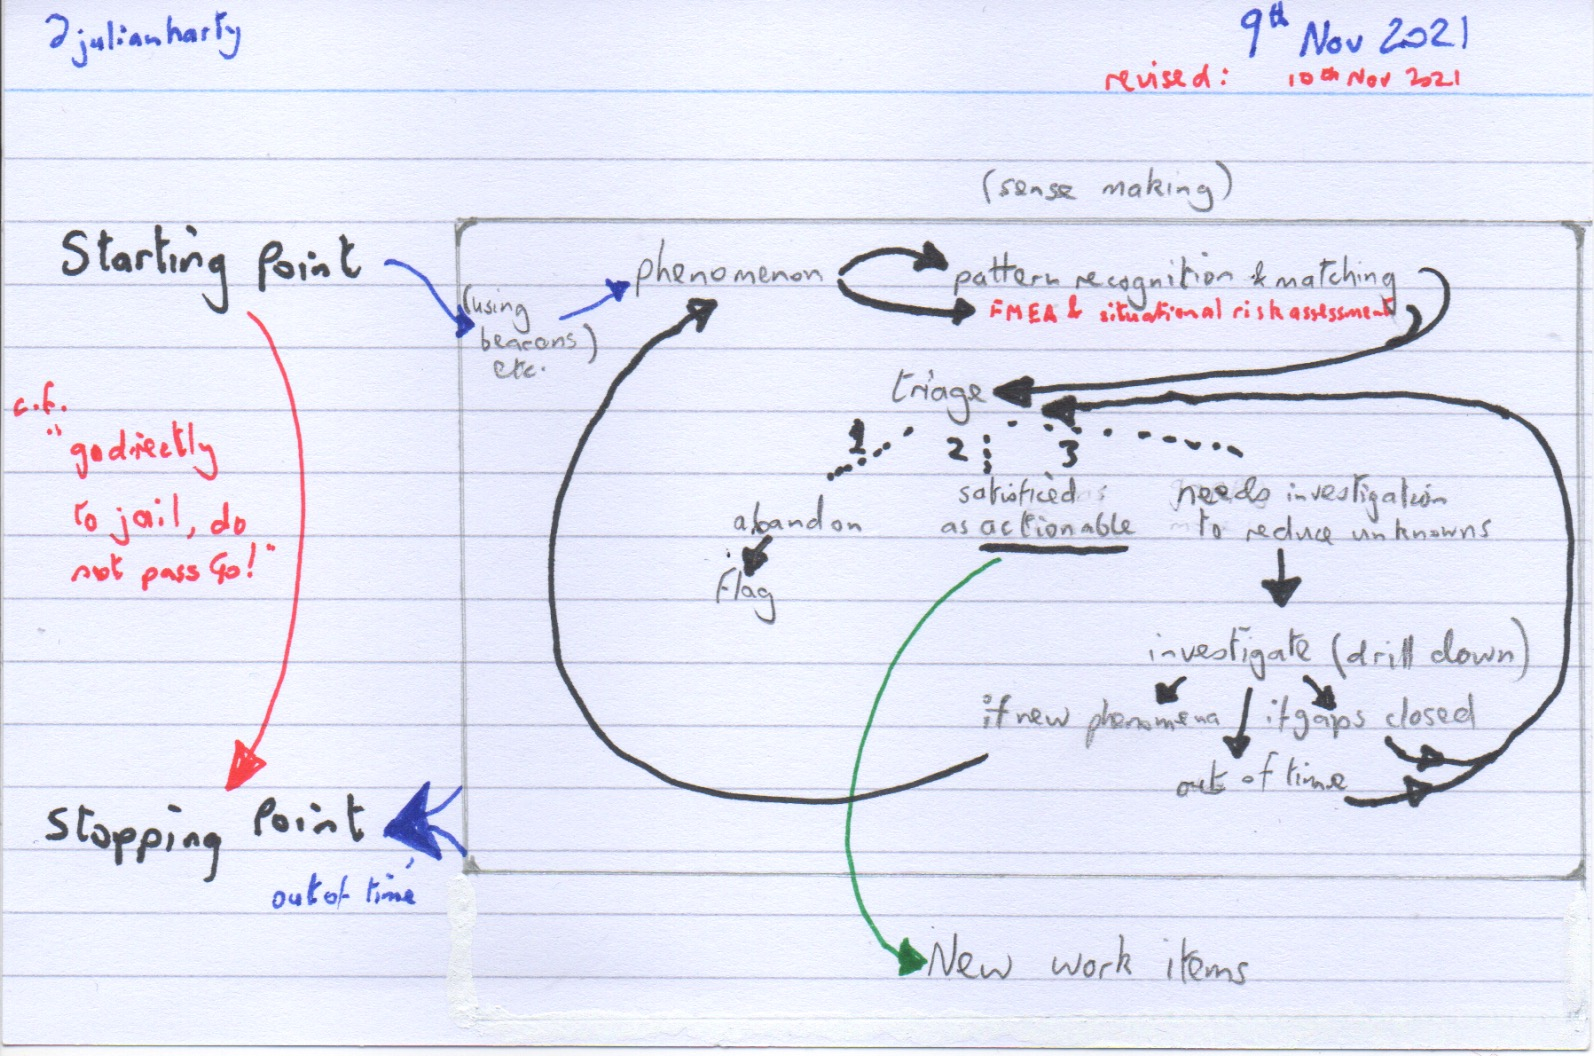
\includegraphics[width=15cm]{images/rough-sketches/practical-sense-making-process-10-nov-2021.jpeg}
    \caption{Sense-making process when development teams apply mobile analytics}
    \label{fig:practical-sense-making-process-when-dev-teams-apply-mobile-analytics}
\end{figure}


Figure~\ref{fig:practical-sense-making-process-when-dev-teams-apply-mobile-analytics} illustrates the sense-making and triage process used by development teams which shares various similarities with sense-making from a research perspective. These similarities mean the researcher and the practitioner may also share similar practices in terms of their analysis of phenomena found in mobile analytics tools. The triage and drill-down may be repeated several times where there is sufficient potential value in performing further investigation. 

The impact of reported failures is combined with situational-risk-assessment as a part of the decision-making process performed by developers during triage; for instance to consider whether this reported issue is worth addressing in the current development cycle, (\textit{e.g.} in the current sprint for teams who use sprints for work planning. Developers have to consider multiple criteria including personal, project, and product implications of making code and/or operational changes. An untested hypothesis for their approach is introduced in the discussion chapter on page \pageref{discussion-decision-making-by-dev-teams-section}.

\newthought{Premature satisfaction}

Many of the developers were often satisficed with what the mobile analytics tools reported - where they accepted local optima (determined through a combination of observation and asking the app devs), \textit{e.g.} they accepted the `top' crash cluster as the worst one. Therefore, if there are flaws in what is being reported the effects of those flaws may permeate into the results of what the developers \textit{do} and \textit{don't} do. 




\section{Integration}
\julian{Include pipelines, tracking the source of issues including re-visiting integration into the triage process, trusting the tools, ...}

\subsection{Using issue databases}
The GTAF team create issues in their online issue database \url{https://gitlab.com/greentech/} for crashes and include links to the source information in the respective mobile analytics tool. These links are a) only available to people who already have access to the mobile analytics account, and b) are ephemeral.



\newthought{Longer-term adoption and use of mobile analytics}

For the Pocket Code app, there has been an intermittent focus on addressing the causes of failures being reported by the mobile analytics tools. One of the main reasons given by the project leadership was the loss of the product owner who successfully completed his PhD and moved to a role in Industry. 


\section{Discussion on the use of mobile analytics}

% The following either needs connecting to the previous material or relocating to later in this chapter where we discuss pii and ethics.
For the Catrobat case study, the project leadership saw sufficient benefits from using mobile analytics after the hackathon that they decided to also implement it in the iOS app. They subsequently reverse this decision because of the intrusive data collection collected implicitly by Firebase Crashlytics. This topic is discussed later in chapter.\pending{Add a forward reference once that material has been added.}

\subsection{What's ``good enough"? and for whom?}